\documentclass{beamer}
\usepackage[utf8]{inputenc}
\usepackage{palatino}
\usepackage{subfig}
\usepackage{amsmath}
\usepackage{amssymb}
\usepackage{dsfont}
\usepackage{multimedia}
\usepackage{hyperref}

\usetheme{Warsaw}
\usecolortheme{crane}

% www.sharelatex.com/learn/Beamer

\title{Computing Entropies with Nested Sampling}
\author{Brendon J. Brewer}
\institute{Department of Statistics\\
The University of Auckland}
\date{\color{blue}\url{https://www.stat.auckland.ac.nz/~brewer/}}

\begin{document}

\frame{\titlepage}


% New slide
\begin{frame}
\frametitle{What is entropy?}

Firstly, I'm talking about information theory, not thermodynamics (though the
two are connected).

\end{frame}


% New slide
\begin{frame}
\frametitle{Shannon entropy}

Consider a discrete probability distribution with probabilities
$\boldsymbol{p} = \{p_i\}$. The Shannon entropy is
\begin{align}
H(\boldsymbol{p}) &= -\sum_i p_i \log p_i
\end{align}

It is a real-valued property of the distribution.

\end{frame}



% New slide
\begin{frame}
\frametitle{Relative entropy}

Consider two discrete probability distributions with probabilities
$\boldsymbol{p} = \{p_i\}$ and $\boldsymbol{q} = \{q_i\}$.
The relative entropy is
\begin{align}
H(\boldsymbol{p}; \boldsymbol{q}) &= -\sum_i p_i \log\left(\frac{p_i}{q_i}\right)
\end{align}
Without the minus sign,
it's the `Kullback-Leibler divergence', and is more fundamental than the
Shannon entropy. With uniform $\boldsymbol{q}$, it reduces to the Shannon
entropy (up to an additive constant).
\end{frame}


% New slide
\begin{frame}
\frametitle{Entropy quantifies uncertainty}
If there are just $N$ equally likely possibilities,
i.e., $p_i = 1/N$, then $H = \log N$. \vspace{0.5em}

\begin{center}
\includegraphics[width=0.6\textwidth]{entropy1.pdf}
\end{center}

\end{frame}


% New slide
\begin{frame}
\frametitle{Entropy quantifies uncertainty}
If there are just $N$ equally likely possibilities,
i.e., $p_i = 1/N$, then $H = \log N$. \vspace{0.5em}

\begin{center}
\includegraphics[width=0.6\textwidth]{entropy2.pdf}
\end{center}

\end{frame}

% New slide
\begin{frame}
\frametitle{Entropy quantifies uncertainty}
If there are just $N$ equally likely possibilities,
i.e., $p_i = 1/N$, then $H = \log N$. \vspace{0.5em}

\begin{center}
\includegraphics[width=0.6\textwidth]{entropy3.pdf}
\end{center}

\end{frame}


% New slide
\begin{frame}
\frametitle{What about densities?}
We get `differential entropy'

\begin{align}
H = - \int_{\textnormal{all }x} f(x) \log f(x) \, dx
\end{align}

This generalises log-volume, as defined {\bf with respect to} $dx$.

\begin{alertblock}{Important}
Differential entropy is {\em coordinate-system dependent}.
\end{alertblock}

\end{frame}






% New slide
\begin{frame}
\frametitle{Some entropies in Bayesian statistics}
Written them in terms of parameters $\theta$ and data
$d$, for Bayesian purposes.

\begin{enumerate}
\item<2-> Entropy of the prior for the parameters $H(\theta)$
\item<3-> Entropy of the conditional prior for the data $H(\theta | d)$
\item<4-> Entropy of the posterior $H(\theta | d)$
\item<5-> Entropy of the prior for the data $H(d)$
\end{enumerate}

\end{frame}


% New slide
\begin{frame}
\frametitle{Some entropies in Bayesian statistics}

\begin{block}{Remark}
{\em Conditional entropies} such as (2) and (3)
are defined using an expectation over the quantity conditioned upon.
\end{block}

\end{frame}

% New slide
\begin{frame}
\frametitle{Interpretation of conditional entropies}

How uncertain would the question ``what's the value of $\theta$,
precisely?'' be if the question ``what's the value of $d$, precisely''
were to be resolved?

\end{frame}



% New slide
\begin{frame}
\frametitle{Connections}

Entropy of the joint prior:
\begin{align}
H(\theta, d) &= H(\theta) + H(d | \theta) \\
                          &= H(d) + H(\theta | d).
\end{align}

Mutual information:
\begin{align}
I(\theta; d) &= H(\theta) - H(\theta | d).
\end{align}
This quantifies dependence --- or more fundamentally,
relevance, or the potential for learning.


{\tiny There are many other ways of expressing $I$.}

\end{frame}


% New slide
\begin{frame}
\frametitle{Pre-data considerations}

We might want to know {\em how relevant the data is to the parameters},
before learning the data. We might want to optimise that quantity for
experimental design. But it's nasty, especially if there's nuisance
parameters.
\end{frame}


% New slide
\begin{frame}
\frametitle{Hard integrals}

E.g.
\begin{align}
H(\theta|d) &= -\int p(d) \int p(\theta|d) \log p(\theta|d) \, d\theta \, dd \\
            &= -\int p(d) \int p(\theta|d)
                    \log\left[\frac{p(\theta)p(d|\theta)}{p(d)}\right] \, d\theta \, dd
\end{align}

But $p(d)$, sitting there inside a logarithm, is already supposed to be
a hard integral (the marginal likelihood / evidence)...

\begin{align}
p(d) &= \int p(\theta) p(d|\theta) \, d\theta
\end{align}

\end{frame}


% New slide
\begin{frame}
\frametitle{Marginal Likelihood Integral}
Nested Sampling was invented in order to do this hard integral
\begin{align}
p(d) &= \int p(\theta) p(d|\theta) \, d\theta
\end{align}

or
\begin{align}
Z &= \int \pi(\theta) L(\theta) \, d\theta
\end{align}
where $\pi=$ prior, $L=$ likelihood.
It's just an expectation. Why is it hard?
\end{frame}


% New slide
\begin{frame}
\frametitle{Simple Monte Carlo fails}

\begin{align}
Z &= \int \pi(\theta) L(\theta) \, d\theta \\
  &\approx \frac{1}{N} \sum_{i=1}^N L(\theta_i)
\end{align}
with $\theta_i \sim \pi$ will probably miss the
tiny regions where $L$ is high.

Equivalently, $\pi$ implies a {\em very heavy-tailed}
distribution of $L$-values, and simple Monte Carlo fails.

\end{frame}


% New slide
\begin{frame}
\frametitle{Nested Sampling}
Nested Sampling takes the original problem and constructs
a 1D problem from it.

\begin{align}
Z = \int_0^1 L(X) dX
\end{align}
where
\begin{align}
X(\ell) &= \int_{L(\theta) > \ell} \pi(\theta) \, d\theta
\end{align}

\begin{block}{The meaning of $X$}
$X(\ell)$ is the amount of prior mass whose likelihood exceeds
$\ell$. As $\ell$ increases, $X$ decreases.
\end{block}

\end{frame}


\begin{frame}
\frametitle{Nested Sampling}

\begin{center}
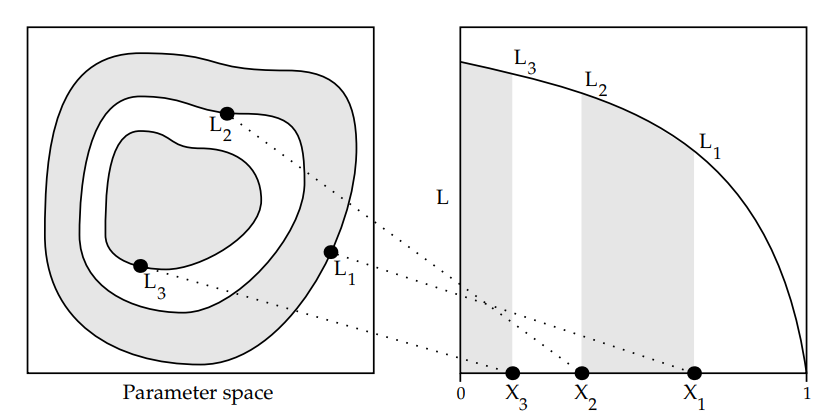
\includegraphics[width=0.8\textwidth]{skilling.png}

Figure from Skilling (2006).
\end{center}

Since $X(\ell)$ is the CDF of $L$-values implied by $\pi$,
points $\theta \sim \pi$ have a uniform distribution over $X$.

\end{frame}



% New slide
\begin{frame}
\frametitle{Nested Sampling}
The idea is to generate a sequence of points with increasing
likelihoods, such that we can estimate their $X$ values. Since
we know their $L$-values, we can then do the integral 
numerically.

\begin{align}
Z = \int_0^1 L(X) dX
\end{align}

\end{frame}


% New slide
\begin{frame}
\frametitle{Nested Sampling algorithm}

\begin{enumerate}
  \item<2-> Generate $N$ points from $\pi$
  \item<3-> Find the worst one (lowest likelihood $L^*$), save it
  \item<4-> Estimate its $X$ using Beta$(N,1)$ distribution\footnote{From order statistics.}
  \item<5-> Record worst particle and its $X$-value, then discard it.
  \item<6-> Replace that point with a new one from $\pi$ but with
        likelihood above $L^*$.
  \item<7-> Repeat steps 2--5 indefinitely.
\end{enumerate}
\end{frame}


% New slide
\begin{frame}
\frametitle{The sequence of $X$-values}
The sequence of $X$ values, if you transform them, have
a Poisson process distribution with rate $N$.

\begin{align}
-\ln(X_1) &\sim \textnormal{Exponential}(N) \\
-\ln(X_2) &\sim -\ln(X_1) + \textnormal{Exponential}(N) \\
-\ln(X_3) &\sim -\ln(X_2) + \textnormal{Exponential}(N) 
\end{align}

(forgive the notational abuse)

\end{frame}

% New slide
\begin{frame}
\frametitle{Poisson process view of NS}

The number of NS iterations taken
to enter a small region (defined by a likelihood threshold) 
as an unbiased estimator of the log-probability
of that region!\vspace{0.7em}

Also, $\pi(\theta)$ can be any distribution (needn't be
a prior) and $L(\theta)$ any scalar function. Opportunities here...

\end{frame}


% New slide
\begin{frame}
\frametitle{My algorithm}
To compute $H(\theta) = -\int f(\theta) \log f(\theta) \, d\theta$
when $f$ can be sampled but not evaluated:

\begin{enumerate}
  \item<2-> Generate a `reference point' $\theta_{\rm ref}$ from $f$
  \item<3-> Do a Nested Sampling run with $f$ as ``prior'' and
            minus the distance to $\theta_{\rm ref}$ as
            ``likelihood''.
  \item<4-> Measure how many NS iterations were needed to make the
            distance to $\theta_{\rm ref}$ really small, and divide
            by $N$. That gives an
            unbiased estimate of the
            log-prob near $\theta_{\rm ref}$.
  \item<5-> Repeat steps 1--3 many times.
  \item<6-> Average the estimated log-probs, then apply corrections
            to convert to density.
\end{enumerate}
\end{frame}


% New slide
\begin{frame}
\frametitle{Paper and software}

{\color{blue}\url{http://www.mdpi.com/1099-4300/19/8/422}
\url{https://github.com/eggplantbren/InfoNest}}
\vspace{0.5cm}

\begin{center}
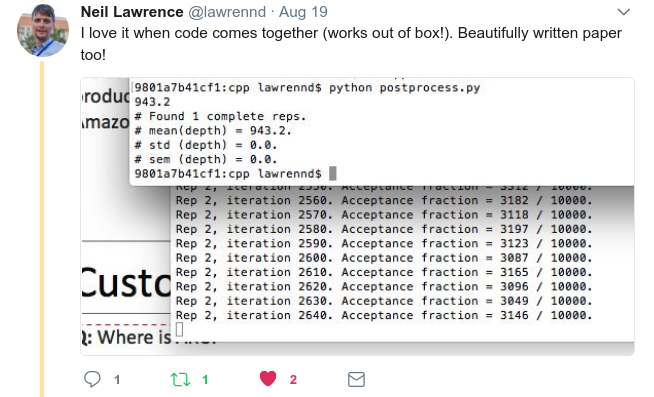
\includegraphics[width=0.7\textwidth]{lawrence.png}
\end{center}

\end{frame}





% New slide
\begin{frame}
\frametitle{References I.}

On the connection between Shannon entropy and thermodynamic entropy,
see: \vspace{2em}

{\tiny Jaynes, Edwin T. ``Gibbs vs Boltzmann entropies.''
American Journal of Physics 33, no. 5 (1965): 391-398. \\

Brewer, Brendon J. ``Unscrambling the Second Law of Thermodynamics''
{\color{blue}
  \url{https://quillette.com/2016/01/28/unscrambling-the-second-law-of-thermodynamics}
}
} % tiny

\end{frame}

%% New slide
%\begin{frame}
%\frametitle{Statements and questions}
%Consider a problem with three mutually exclusive, exhaustive possibilities
%\texttt{a}, \texttt{b}, and \texttt{c}.


%\begin{center}
%  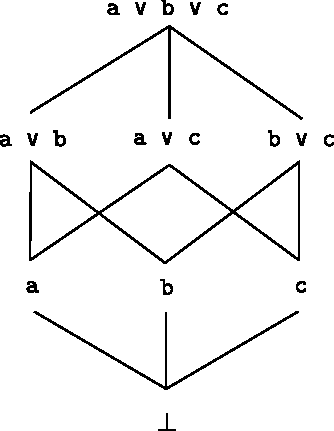
\includegraphics[width=0.3\textwidth]{lattice1.pdf}
%\end{center}

%\end{frame}



\end{document}


